\chapter{Markov chains}

\textit{"Some type of an automata, that represent probability space. It needs to have special properties."}

\begin{figure}[!h]\centering
	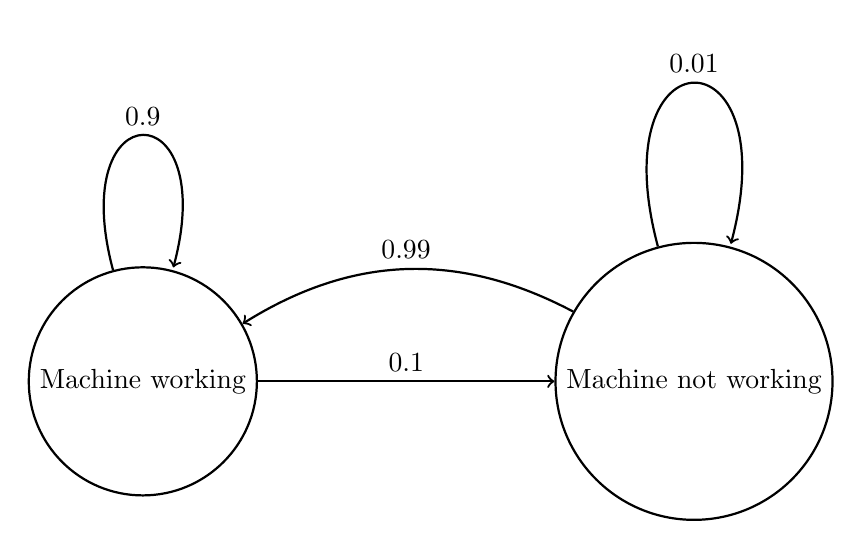
\begin{tikzpicture}[node distance={70mm}, thick, main/.style = {draw, circle}]
		\node[main] (1) {Machine working};
		\node[main] (2) [right of=1] {Machine not working};
		\path
			(1) edge [loop above] node {$0.9$} (1)
			(2) edge [loop above] node {$0.01$} (2);
		\path
			(1) edge [->] node [above] {$0.1$} (2)
			(2) edge [->] [bend right] node [above] {$0.99$} (1);
	\end{tikzpicture}
	\caption{Example of a Markov chain.}
	\label{markov-chain}
\end{figure}

\section{Model}

\begin{itemize}
	\item States: $S$ it is usually finite and sometimes only countable.
	\item sequence $X_{0}, X_{1}, X_{2}, \dots$ of random variables with values in $S$
	\item $X_{t+1}$ depends \textbf{only} on $X_{t}$
	\item $\Pr [X_{t+1} = j \vert X_{t} = i] = p_{ij}$ where $i,j \in S$
\end{itemize}

\begin{defn}
	Sequence of r.v. $X_{0},X_{1},X_{2},\dots$ is a \textbf{Markov chain} if:
	
	\begin{itemize}
		\item $\exists$ countable $S : \text{Rng } X_{t} \subset S$  $\forall t$
		\item $\forall t \in \mathbb{N}$ $\forall a_{0}, a_{1}, a_{2}, \dots , a_{t+1} \in S$
	\end{itemize}
	
	$$
	\Pr[X_{t+1} = a_{t+1} \vert X_{0} = a_{0}, X_{1} = a_{1} , \dots ,X_{t} = a_{t}] = \Pr [X_{t+1} = a_{t+1} \vert X_{t} = a_{t}]
	$$
\end{defn}

This means that Markov chain has the property of being memory-less and this probability written above is called \textit{transition probability}. We can map all elements from $S$ to a number from range $1,2,\dots ,n$ and then we can build \textbf{transition matrix}.

$$
P =
\begin{pmatrix}
p_{11} & p_{12} & p_{13} & \dots \\
p_{21} & p_{22} &  \\
p_{31} &  & \ddots \\
\vdots
\end{pmatrix}
$$

Where $p_{ij}$ means going from $i$ to $j$. All $p_{ij} \geq 0$ and the sum of each row is $1$. Also we can build \textbf{transition graph} representing this Markov chain. In that graph $V = S$ and arcs exists if $(ij) : p_{ij} > 0$.

Now we look at distribution, or PMF of $X_{k} = \pi^{(k)}$ where $\pi^{(k)} = \left( \pi_{1}^{(k)}, \pi_{2}^{(k)},\pi_{3}^{(k)}, \dots \right)$ and the sum is $1$. Then we may see that $\pi_{j}^{(k)} = \Pr[X_{k} = j]$. We will be calling $\pi^{(0)}$ an \textit{initial state}.

Then we can see that $\pi^{(1)} = \pi^{(0)} P$ as multiplication by transition matrix. We can generalize this to:

$$
\pi^{(k)} = \pi^{(k-1)} P
$$

\begin{thm}
	For any \textit{MC} with transition matrix $P$ we have $\pi^{(k)} = \pi^{(0)} P^{k}$ and $\pi^{(k+1)} = \pi^{(t)} P^{k}$.
\end{thm}

\begin{proof}
	Proof will be by induction. So $\pi^{(k+1)} = \pi^{(k)} P = \pi^{(0)} P^{k} P =\pi^{(0)} P^{k+1}$.
\end{proof}

\begin{defn}
	\textbf{K-step transition} is defined as:

	$$
	\begin{array}{rcl}
	r_{ij}(k) & := & \Pr[\text{from }i \text{ to } j \text{ in } k \text{ steps}] \\
	& = & \Pr[X_{k} = j \vert X_{0} = i] \\
	& = & \Pr[X_{t+k} = j \vert X_{t} = i] \\
	r_{ij}(1) & = & p_{ij}
	\end{array}
	$$
\end{defn}

\begin{observ}
	$$
	r_{ij}(k) = \pi_{j}^{(k)} \text{ if } \pi^{0} = \left( 0, 0, \dots, 0, 1, 0 \dots, 0\right)
	$$
	
	Where $1$ is on $i$-th position. Also:
	
	$$
	\pi_{j}^{(k)} = (\pi^{0} P^{k})_{j} = \left( \left( 0, 0, \dots, 0, 1, 0 \dots, 0\right)P^{k}\right)_{j} = (P^{k})_{ij}
	$$
\end{observ}

\section{Chapman-Kologorov formula}

$$
\begin{array}{r c l}
	r_{ij}(k) & = & (P^{k})_{ij} \\
	r_{ij}(k+l) & = & \sum_{t=1}^{S} r_{it}(k)r_{tj}(l) \\
	r_{ij}(k+1) & = & \sum_{t=1}^{S} r_{it}(k) p_{tj}
\end{array}
$$

\begin{defn}
	$j$ is \textbf{accessible} from $i$ if
	
	$$
	\begin{array}{c}
		(j \in A(i), i \to j) \\
		\Updownarrow \\
		\Pr[\exists k \geq 0 : X_{k} = j \vert X_{0} = i] > 0 \\
		\Updownarrow \\
		\sum_{k=0}^{\infty} r_{ij}(k) > 0 \\
		\Updownarrow \\
		\exists \text{ a discrete path from } i \text{ to } j \\
		\text{in the transition graph}
	\end{array}
	$$
\end{defn}

\begin{defn}
	$i$ and $j$ from $S$ are \textbf{commuting states} $(i \leftrightarrow j)$ iff $i \to j$ and $j \to i$.
\end{defn}

\begin{lemma}
	$\leftrightarrow$ is an equivalence relation.
\end{lemma}

\begin{proof}
	We need to show that it satisfies reflexivity, symmetry and transitivity.
	
	\begin{enumerate}
		\item $i \leftrightarrow i$ which means $i \to i$ so $r_{ii}(0) =1$
		\item $i \leftrightarrow j$ iff $j \leftrightarrow i$ by definition
		\item $i \leftrightarrow j$ and $j \leftrightarrow t$ we want to show $i \leftrightarrow t$, but we know $i \to j \to t$ and $t \to j \to i$ so we use these paths (or just shorten them by first intersection).
	\end{enumerate}
\end{proof}

\begin{defn}
	An \textbf{equivalence class} in a Markov chain is a set of states that are commuting with each other. The set is maximal with its property. In other words, no additional state from $S$ can be included in the set without breaking the commuting property.
\end{defn}

\begin{defn}
	\textit{MC} is called \textbf{irreducible} if $\leftrightarrow$ has just $1$ equivalence class. This is equivalent to that $\forall ij : i \leftrightarrow j$.
	
	Or by graph theory we can say that the transition graph is strongly connected and when we compress these classes we get DAG.
\end{defn}

\begin{defn}
	$i \in S$ is called \textbf{recurrent} if $\forall j \in A(i) : i \in A(j)$ and \textbf{transient} otherwise.
\end{defn}

\begin{thm}
	$i \in S$ we define $f_{ii} = \Pr[\exists t \geq 1 : X_{t} =i \vert X_{0} = i]$ or by words "probability of going back to $i$". Then:
	
	\begin{itemize}
		\item $i$ is recurrent iff $f_{ii} = 1$
		\item $i$ is transient iff $f_{ii} < 1$
	\end{itemize}
\end{thm}

\begin{proof}
	$i$ is transient iff $\exists j \in A(i) : i \notin A(j)$. Starting with $X_{0} = i$ the probability $\exists t \geq 1 : X_{t} = j$ is $p > 0$ and $\Pr[\text{going to } i \text{ from } j] = 0 \Rightarrow f_{ii} \leq 1 - p$. And if $i$ is recurrent then $f_{ii} = 1$.
\end{proof}

\begin{defn}
	$i \in S$ we define $V_{i}$ as number of visits to $i$ or written as $|\{t : X_{t} = i\}|$
	
	$V_{i} \in \mathbb{N} \cup \{\infty\}$ so it is a random variable defined by $X_{0}, X_{1}, \dots$
\end{defn}

\begin{thm}
	$i$ is recurrent $\Rightarrow \Pr[V_{i} = \infty | X_{0} = i] = 1$
	
	$i$ is transient $\Rightarrow (V_{i} \vert X_{0}= i) \sim \text{Geom}(1 - f_{ii})$, where $(1-f_{ii})$ is called as \textit{escape probability}.
\end{thm}

\section{Steady state}

\begin{defn}
	Let $\pi$ be a distribution on $S$ such that $\left( \pi_{1} + \pi_{2} + \dots + \pi_{S} = 1, \pi_{i} > 0\right)$. Then $\pi$ is \textbf{stationary} distribution if $\pi P = \pi$. Or can be written as $\left[ \pi = (\pi_{1}, \pi_{2}, \dots) \vert \forall j \pi_{j} = \sum_{i \in S} \pi_{i} p_{ij}\right]$ for \textit{MC} with transition matrix $P$.
\end{defn}

\begin{observ}
	If $\pi^{(0)} = \pi$ and $\pi$ is stationary then $\pi^{(1)} = \pi$ and $\forall k : \pi^{(k)} = \pi$.
\end{observ}

\begin{defn}
	$s \in S$ is \textbf{periodic} if $\exists \Delta \geq 2$ integer such that $\Pr[X_{t} = s \vert X_{0} = s] > 0 \Rightarrow \Delta \vert t$. \textit{MC} is periodic if all its states are periodic, otherwise it is \textit{aperiodic}.
\end{defn}

\begin{thm}
	$(X_{t})_{t = 0}^{\infty}$ is a \textit{MC} that is \textit{irreducible}, \textit{aperiodic} and $|S| < \infty$. Then $\exists \pi$ that is a stationary distribution and $\forall j \forall i \lim_{k\to\infty}r_{ij}(k) = \pi_{j}$, $\pi$ is a unique solution to
	
	$$
	\pi P = \pi
	$$
	
	$$
	\pi \mathbf{1} = 1
	% vector of 1s
	% TODO: I think this is wrong. Pi is a probability distribution, so if pi_j is 1, then all other indexes must be 0.
	$$
\end{thm}

\section{Absorption probability}

\begin{defn}
	Absorption states are such states, that the probability of staying in the same state is $1$. Or it is $\{s \in S : p_{ss} = 1\}$.
\end{defn}



\begin{lemma}[Probability of Absorption]
	Assume a \textit{MC} with absorbing state $0$ (and some move). Put
	
	$$
	a_{i} = \Pr[\exists t : X_{t} = 0 \vert X_{0} = i] \text{ for } i \in S
	$$
	
	Then $(a_{i})$ are the unique solution to:
	
	$$
	\begin{array}{rcll}
		a_{0} & = & 1 \\
		a_{i} & = & 0 &\text{ if } i \neq 0 \text{ and absorbing} \\
		a_{i} & = & \sum_{j \in S} p_{ij} a_{j} & \text{ for } i \text{ not absorbing}
	\end{array}
	$$
\end{lemma}

\begin{proof}
	$a_{0} = 1$ and $a_{i} = 0$ if $i \neq 0$ and absorbing is easy observation. Lets assume $i$ is not absorbing then
	
	$$
	\begin{array}{r c l}
		a_{i} & = & \Pr[\exists t : X_{t} = 0 \vert X_{0} = i] = \\
		& = & \sum_{j \in S} \Pr[X_{1} = j \vert X_{0} = i] \cdot \Pr[\exists t : X_{t} = 0 \vert X_{0} = i, X_{1} = j] = \\
		& = & \sum_{j \in S} p_{ij} \Pr[\exists t : X_{t} = 0 \vert X_{0} = j] = \\
		& = & \sum_{j \in S} p_{ij} a_{j} \\
	\end{array}
	$$
\end{proof}

\section{Mean time to absorption}

$A \subseteq S$ is set of all absorption states. $T = \min \{ t \geq 0 \vert X_{t} \in A\}$ is \textit{absorption time} and random variable. Then we define $\mu_{i} = \mathbb{E} [T \vert X_{0} = i]$.

\begin{thm}
	$(\mu_{i})_{i \in S}$ is the unique solution to:
	
	$$
	\begin{array}{rrcl}
		\text{if } i \in A & \mu_{i} & = & 0 \\
		\text{if } i \notin A & \mu_{i} & = &1 + \sum_{j \in S} p_{ij}\mu_{j}
	\end{array}
	$$
\end{thm}

\section{SAT}

Problem where there is given a Boolean formula and we have to say if it is satisfiable.

\subsection{2-SAT (polynomial)}

Special case of \textit{SAT} where all clauses have at most $2$ literals.

\subsubsection{Algorithm for 2-SAT}

\begin{enumerate}
	\item Start with any assignment $(x_{1} = x_{2} = \dots = x_{n} = F)$
	\item Repeat up to $2mn^{2}$ times ($n$ is the number of variables and $m$ is an arbitrary parameter)
	\begin{itemize}
		\item if $\varphi$ is satisfiable return "YES"
		\item otherwise, choose any clause that is not satisfied and randomly change one of its variables $(\ast)$
	\end{itemize}
	\item Return "NO"
\end{enumerate}

$Pr[\text{incorrectly saying no}]  \leq \frac{1}{2m}$ which can be proved by Markov inequality.

$Pr[\text{incorrectly saying no}]  \leq \frac{1}{2^m}$ using iterative Markov inequality.

\subsection{3-SAT}

\subsubsection{Algortihm for 3-SAT}

\begin{itemize}
	\item Repeat for $\leq m$ times
	\begin{itemize}
		\item Repeat for $\leq 3^{n/2}$ times
		\begin{itemize}
			\item randomly initialize the variables
			\item if $\varphi$ is satisfiable return "YES"
			\item otherwise, choose any clause that is not satisfied and randomly change one of its variables
		\end{itemize}
	\end{itemize}
\end{itemize}

Running time of this algortihm is exponential in $n$.

$P[\text{failure}] \leq \frac{1}{2^m}$

By using a better algorithm we can get the exponential part to be $\frac{4^n}{3}$.

The idea behind these algorithms is that we are using a \textit{random walk} on the space of all possible assignments. This is a \textit{Markov chain}. So we can easily calculate the probability of getting to the absorbing state and the mean time to get there.
